
\section{Object Oriented}

Object-oriented design is the process of planning a system of interacting objects for the purpose of solving a software problem. It is one approach to software design. An object contains encapsulated data and procedures grouped together to represent an entity. The 'object interface' defines how the object can be interacted with. An object-oriented program is described by the interaction of these objects. Object-oriented design is the discipline of defining the objects and their interactions to solve a problem that was identified and documented during object-oriented analysis.

\iffalse
 basic requirement of this app is that the user must be having ANDROID
Operating System in his phone or tablet. The minimum version of Androids Operating
System must be ICECREAM SANDWICH. All the versions of Android OS above
IcecreamSandwich( i.e. Jellybean, Kitkat, Lollipop,Marshmallows) will support this
app. A user needs Monitary app installed in device .


\noindent As shown in the Figure \ref{fig:1}, .\\Brief introduction showing the features available in the application.

\begin{figure}[ht]
\centering
\includegraphics[scale=0.5]{images/s1.png}
\caption{Screen 1}
\label{fig:1}
\end{figure}

\noindent This are the options the navigation drawer the app will contain. These will contain the screens the user can navigate too that can be seen in Figure \ref{fig:2}. \\

\begin{figure}[ht]
	\centering
	\includegraphics[scale=0.49]{images/s2.png}
	\caption{Screen 2}
	\label{fig:2}
\end{figure}

\noindent  Statistics will be able to change according to the dates selected. Default values will be the current week. User Will be able to see diagrams according to Quantity and
days, Quantity and categories and others.as seen in the Figure \ref{fig:3}.\\

\begin{figure}[ht]
\centering
\includegraphics[scale=0.5]{images/s3.png}
\caption{Screen 3}
\label{fig:3}
\end{figure}

\noindent Reminder view will contain details from the reminder created and the user can edit
the reminder values. in Figure \ref{fig:4}. \\

\begin{figure}[ht]
\centering
\includegraphics[scale=0.38]{images/s4.png}
\caption{Screen 4}
\label{fig:4}
\end{figure}

\noindent Reminder screen will show the current saved Reminder and if they are active or not.
To activate one it will have a switch next to the name so it can be activated in any
moment. The user will be able to erase and add from this view as seen in the Figure \ref{fig:5}. It's named as output.dxf. We can open that file in LibreCAD directly from the command-line.\\


\begin{figure}[ht]
\centering
\includegraphics[scale=0.5]{images/s6.png}
\caption{Screen 5}
\label{fig:5}
\end{figure}

\noindent Expenses View is the main screen that will be showed. The user will be able to add expenses and see a total amount in Today, Week and Month. as shown in Figure \ref{fig:6}. 

\begin{figure}[ht]
\centering
\includegraphics[scale=0.38]{images/s61.png}
\caption{Screen 6}
\label{fig:6}
\end{figure}

\noindent This activity will provide necessary help to the user. One can also mail the maker
(GURNOOR SINGH) for further queries as shown in Figure \ref{fig:7}. 

\begin{figure}[ht]
\centering
\includegraphics[scale=0.38]{images/s7.png}
\caption{Screen 7}
\label{fig:7}
\end{figure}
\noindent User will be able to add and delete categories from the Categories View \ref{fig:8}. 

\begin{figure}[ht]
\centering
\includegraphics[scale=0.38]{images/s8.png}
\caption{Screen 8}
\label{fig:8}
\end{figure}
\fi

\section{Detail Design}

	\subsection{Registration}
	When the user first launches the app he sees the splash screen, if he is not logged in then he will see the login screen, if he hasn't created any account yet then he will have to register first, After submitting details during registration he will recieve an email confirming his email account. On successful email confirmation, he can login in the app. \\
	
	\subsection{Home}
	After Successful login, he will see the home screen, which will be the introduction page of sports department.After that user will have access to the following parts : 
	\begin{itemize}
		\item \textbf{Bottom Slider}:- This part is available in the admin panel application.Under this feature admin has access to add news related to athlatic meet, sports day or any latest information added to the department.Admin also has access to add achievement of students in sports. 
				
		\item \textbf{Navigation Drawer Menu}:- It is the main menu of the app. It opens by left swiping. It contains following options:
		\begin{itemize}
			\item \textbf{Introduction}:- It will give introduction about the sports department.Mission and Vision is also discussed under this pannel.
			
			\item \textbf{Commitee}:- It shows the list of commitee members currently available in the sports department.
			
			\item \textbf{Latest News}:- Here admin can upload the latest news about of the sports department. Admin can also upload image if required with the news.
			
			\item \textbf{Facilities}:-It shows the facilities that sports department of college provide to their students such as gym , cricket groung etc.
			
			\item \textbf{Athletic Meet}:- By Clicking this user will get latest news about athletic meet , results of the athletic meet and also the records made under meet.
			
			\item \textbf{Scholarship}:It shows the scholarships currently available in the college for sports department.
			
			\item \textbf{Analysis}:-It will display the anaylsis part of the participation engineering branches made in a particular year.
			
			\item \textbf{Achievement}:-It will have two options:
			\begin{itemize} 
			\item \textbf{Intramural}:-Achievement of students who participated or got medals in activities or events performed under college boundaries will be displayed here.
			\item \textbf{Extramural}:-Achievement of students who participated or got medals in activities or events performed outside of college boundaries will be displayed here.
			\end{itemize}
			\item \textbf{Communicate}:-
			\begin{itemize} 
			\item \textbf{Contact Us}:-It will display the contacts of sports department.Also Email-Id will be thier of sports department. 
			\item \textbf{Map}:-It will display the map of sports department.
\item \textbf{Share}:-It will help the user to share the application with another member.User can share the application in whatsapp , facebook , messanger etc.
\item \textbf{Developers}:-It will display the information of the developers who developed GNDEC Sports.  			
			
			\end{itemize}
			
		\end{itemize}
	\end{itemize}

\section{System Design}

\newpage
\begin{figure}[ht]
	
	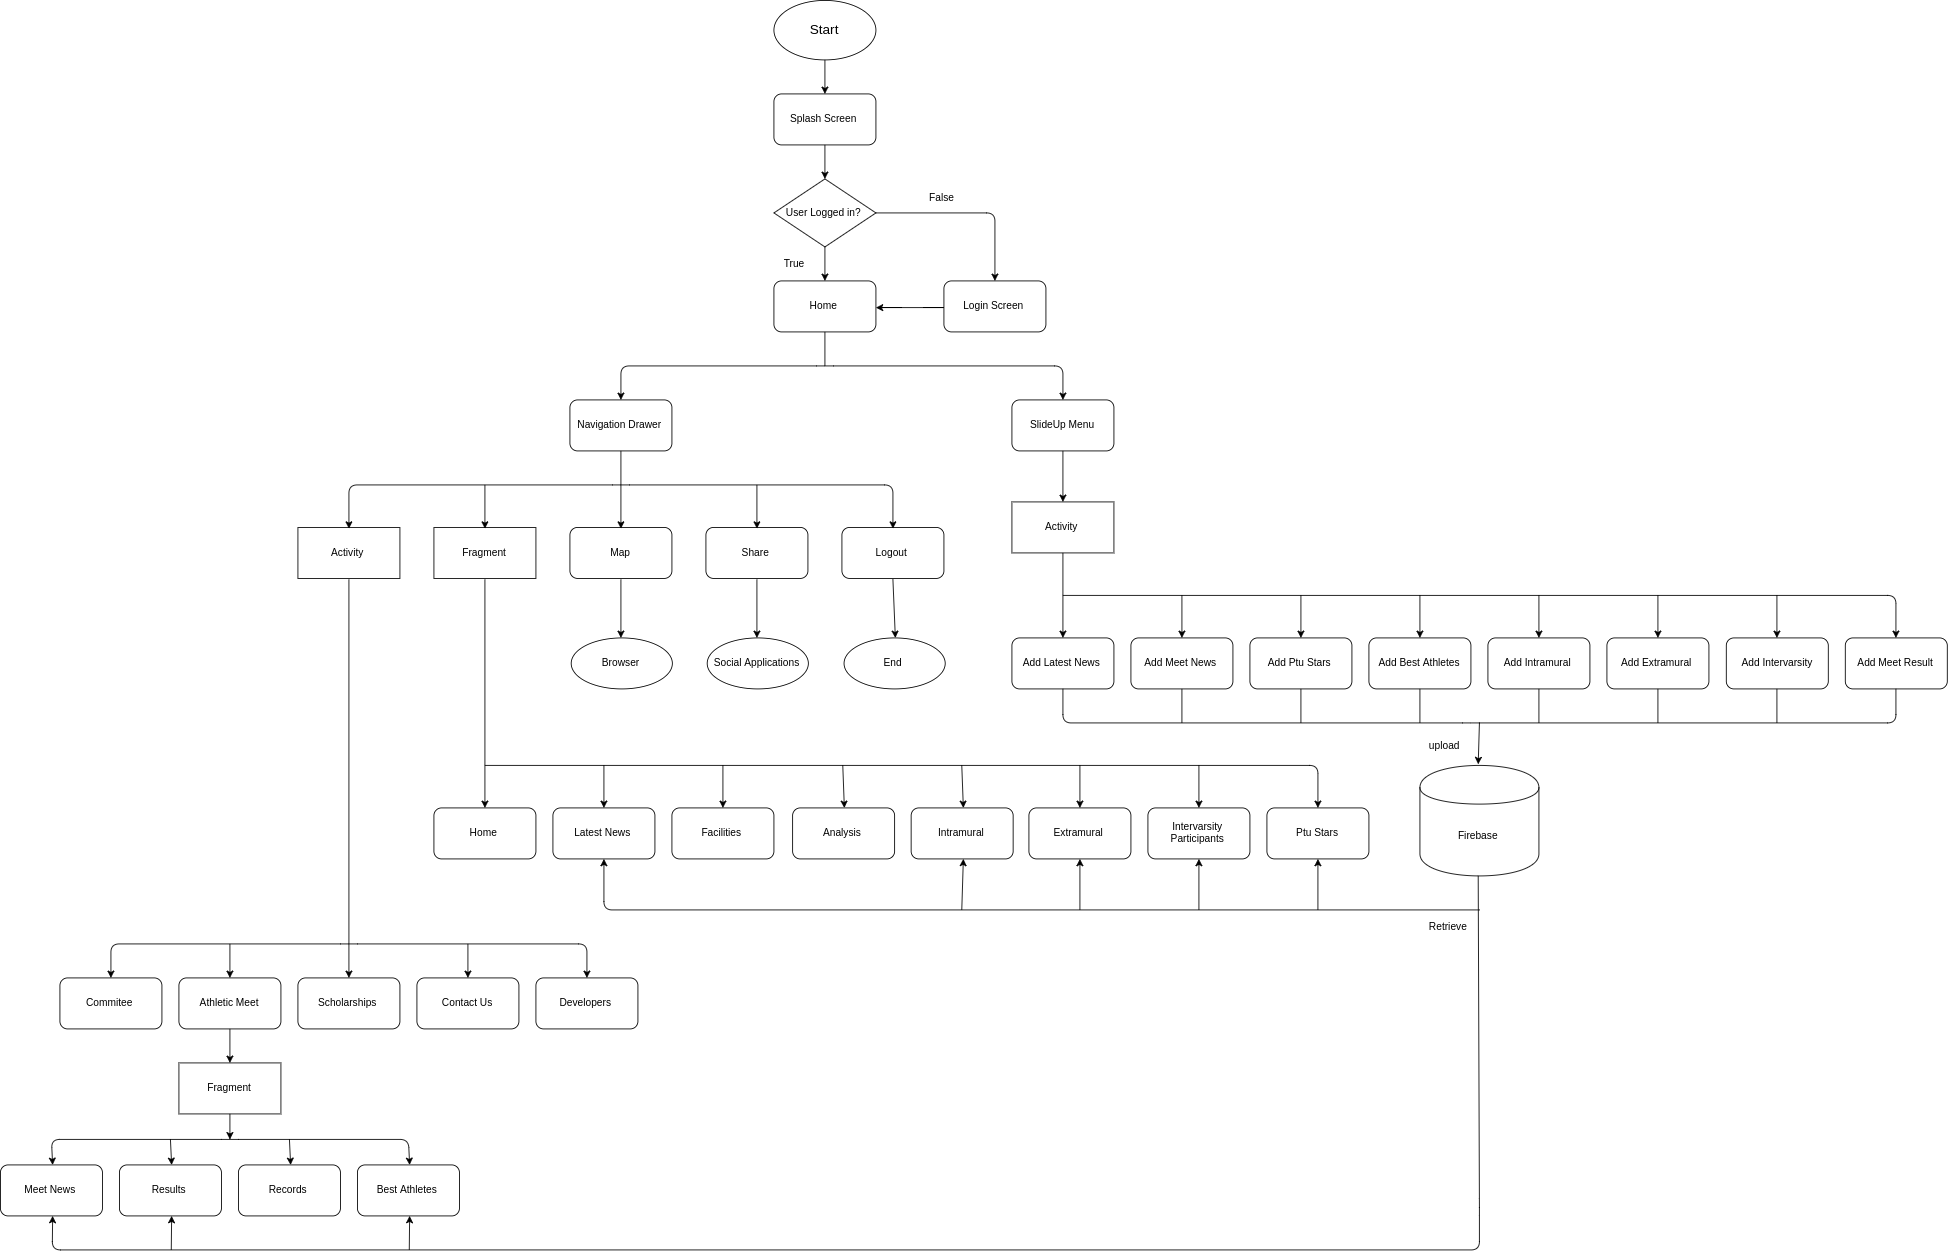
\includegraphics[scale=0.25]{images/Gndecadmingne.png}
	\caption{Flow Chart of gndec admin}
\end{figure}

\newpage
\begin{figure}[ht]
	
	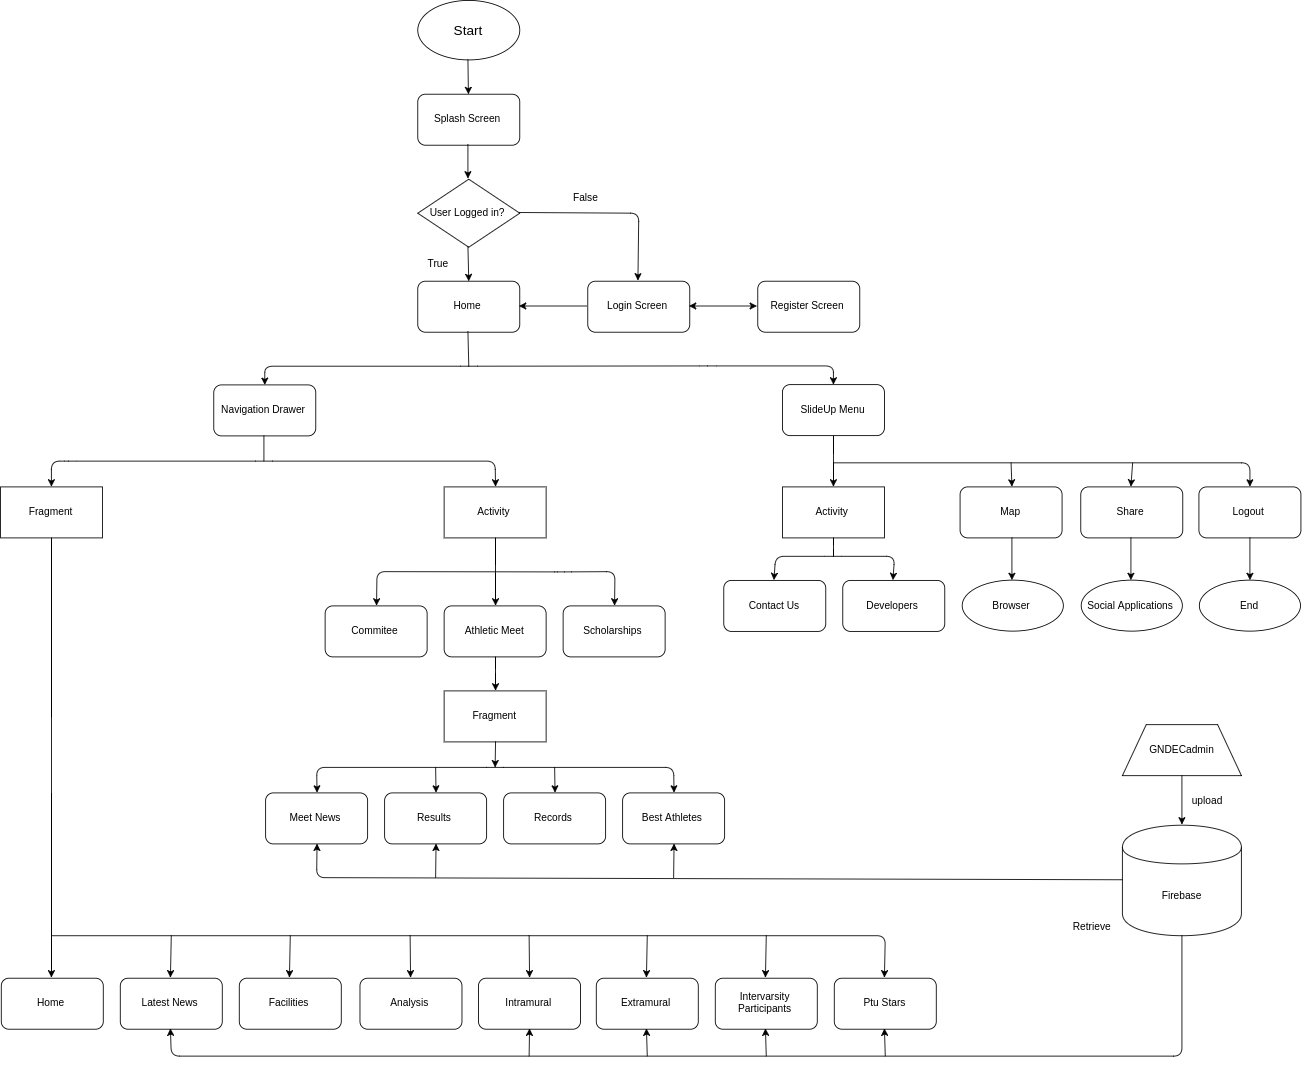
\includegraphics[scale=0.35]{images/Gndecstudent.png}
	\caption{Flow Chart of gndec student}
\end{figure}




\section{Database Design}

\newpage	
	\begin{figure}[ht]
		\centering
		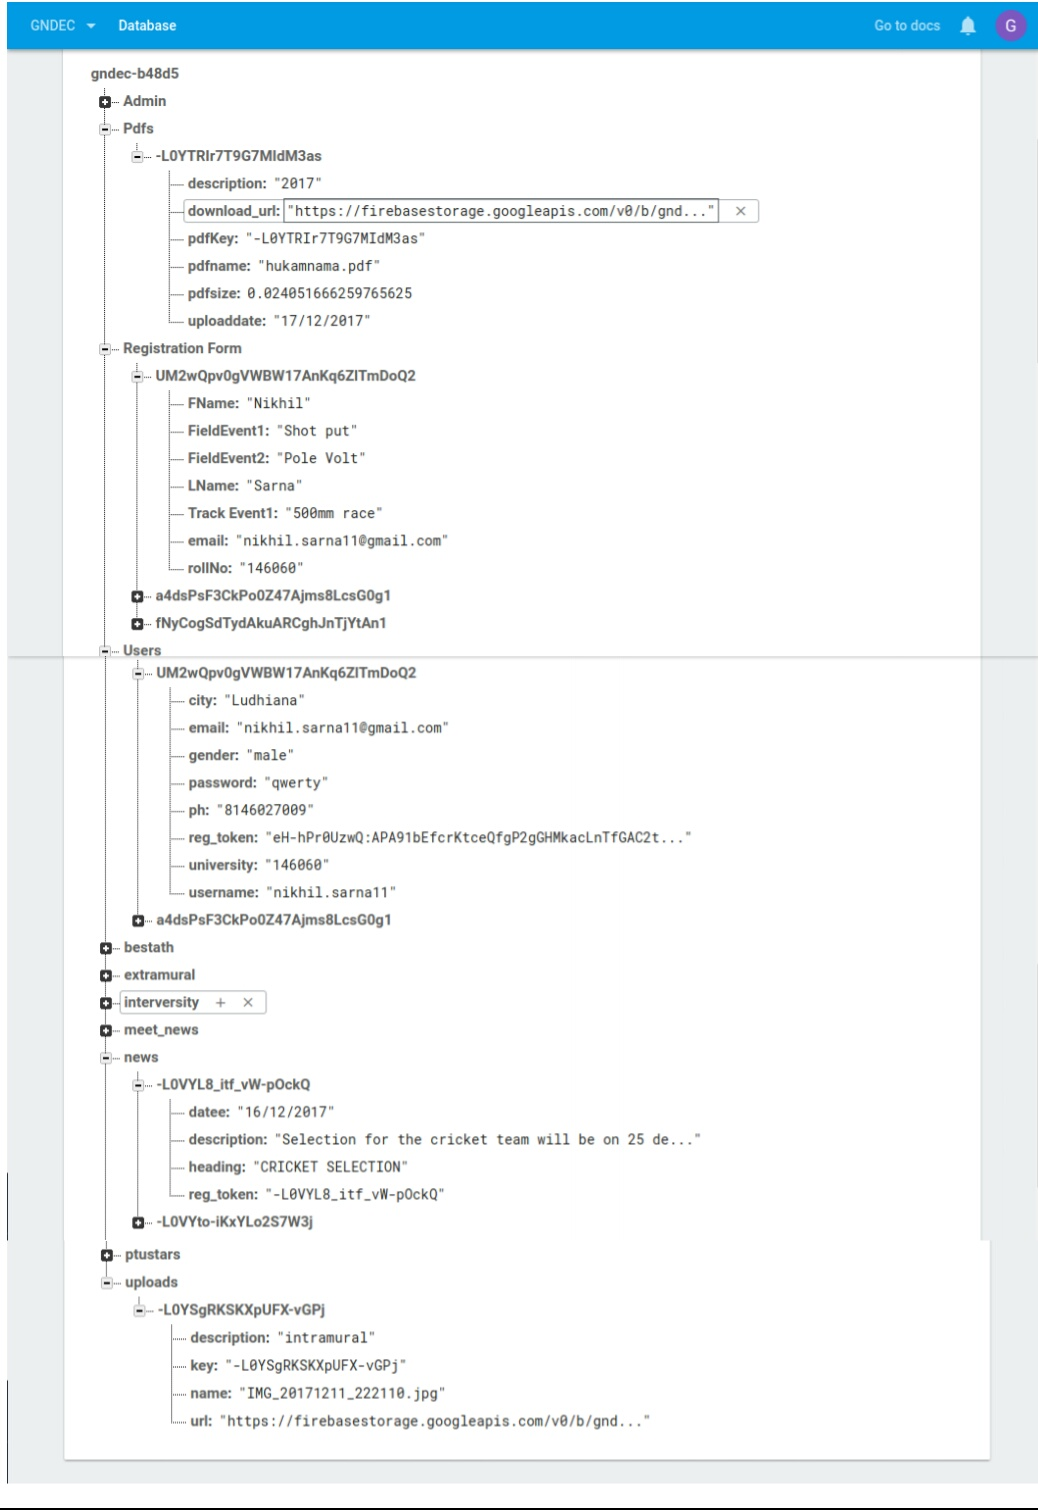
\includegraphics[scale=0.20]{images/dbfire.jpg}
		\caption{ER Diagram}
	\end{figure}

	\subsection{ER Diagram}
	
\newpage	
	\begin{figure}[ht]
		\centering
		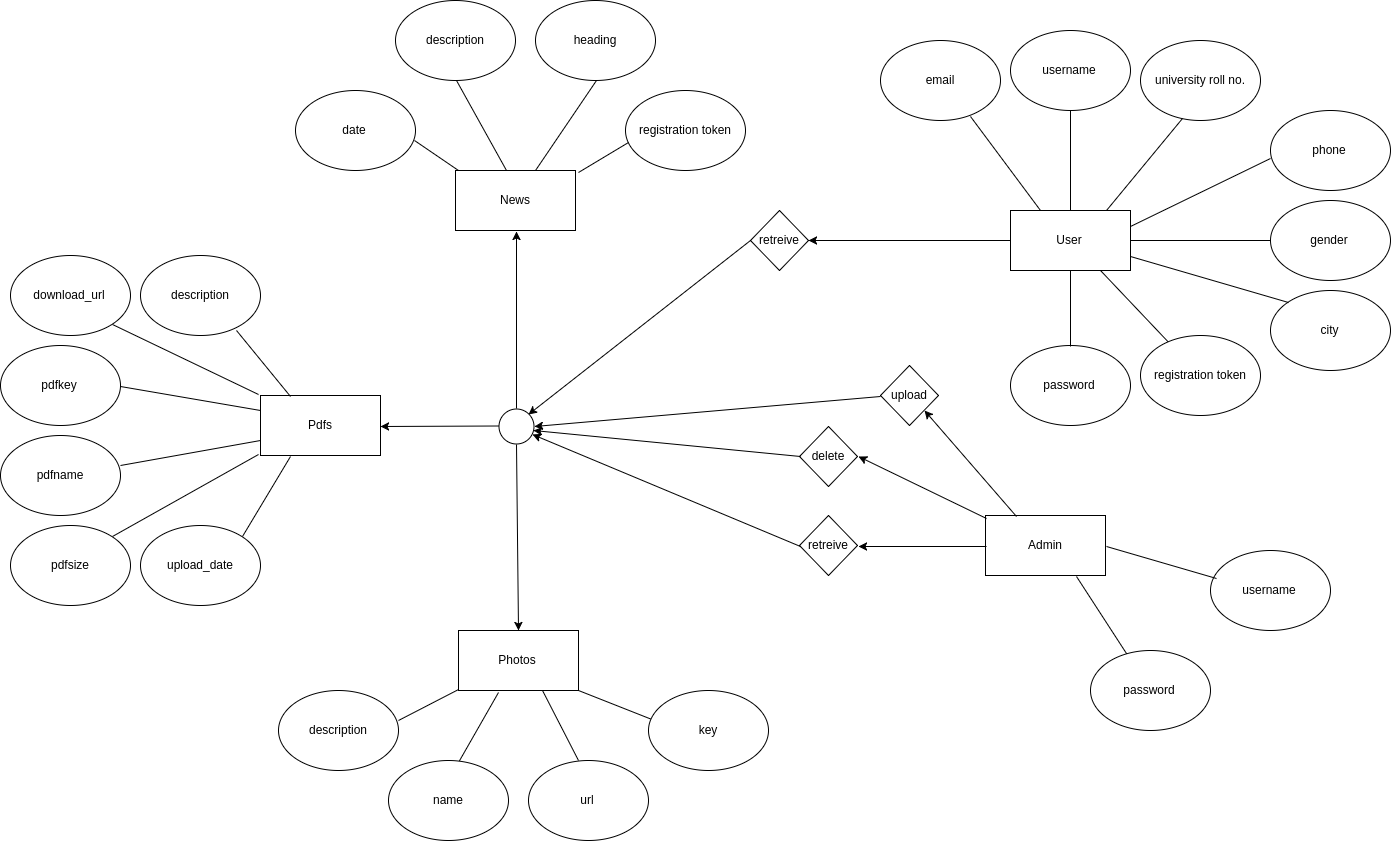
\includegraphics[scale=0.35]{images/ergndec.png}
		\caption{ER Diagram}
	\end{figure}
	
	\subsection{Database Connection Controls and Strings}
	The Firebase Realtime Database is a cloud-hosted database. Data is stored as JSON and synchronized in realtime to every connected client. When we build cross-platform apps with our iOS, Android, and JavaScript SDKs, all of our clients share one Realtime Database instance and automatically receive updates with the newest data. \\
	
	If we are using the latest version of Android Studio (version 2.2 or later), It is recommended using the Firebase Assistant to connect your app to Firebase. The Firebase Assistant can connect our existing project or create a new one for us and automatically install any necessary gradle dependencies.\\
	
	If we are using an older version of Android Studio or have a more complex project configuration, we can still manually add Firebase to our app.
	
		\subsubsection{Using the Firebase Assistant}
		
		To open the Firebase Assistant in Android Studio:
		\begin{itemize}
			\item Click Tools > Firebase to open the Assistant window.
			\item Click to expand one of the listed features (for example, Analytics), then click the provided tutorial link (for example, Log an Analytics event).
			\item Click the Connect to Firebase button to connect to Firebase and add the necessary code to your app.
		\end{itemize}
	
		\subsubsection{Manually adding Firebase}
		To add Firebase to your app you'll need a Firebase project and a Firebase configuration file for your app.
		\begin{itemize}
			\item Create a Firebase project in the Firebase console, if we don't already have one. If we already have an existing Google project associated with our mobile app, click Import Google Project. Otherwise, click Add project.
			\item Click Add Firebase to our Android app and follow the setup steps. If we're importing an existing Google project, this may happen automatically and we can just download the config file.
			\item When prompted, enter our app's package name. It's important to enter the package name our app is using, this can only be set when we add an app to our Firebase project.
			\item At the end, we'll download a google-services.json file. We can download this file again at any time.
		\end{itemize}
